\documentclass{llncs}
% Command to remove the content counter
\setcounter{secnumdepth}{0}

\usepackage[utf8]{inputenc}
\usepackage[T1]{fontenc}
\usepackage[brazilian]{babel}
\usepackage{csquotes}
\usepackage{hyphenat}
\hyphenation{pro-ble-ma}
\usepackage{imakeidx}
\makeindex[columns=3, title=Alphabetical Index, intoc]
\usepackage{enumerate}
\usepackage{amssymb}
\usepackage{amsmath}
\usepackage{array}

% Better handle of numeric things.
% Configured to French style (same 
% as Brazilian conventions)
\usepackage[locale=FR]{siunitx}
\usepackage{hyperref}
\usepackage{graphicx}
\graphicspath{ {images/} }
\usepackage{longtable}
\usepackage{listings}
\setcounter{tocdepth}{1}
\usepackage{tocbibind}

\begin{document}
\begin{titlepage}           
\end{titlepage}
%%%%%%%%%%%%%%%%%%% TITLE PAGE
\begin{titlepage}
  \begin{center}
    \vspace*{1cm}
    %%% TITLE
    \Huge
    \textbf{Tarefa Prática 2}
    \vspace{0.5cm}
    
    %%% CURRICULAR UNIT
    \LARGE
    Modelação e Caracterização de Tráfego
    %%% AUTHORS    
    \vspace{1.0cm}
    \small
    \textbf{\\PG39254 - Igor Araújo\\PG39255 - Matheus Gonçalves\\PG41017 - I-Ping}
    
    %%% LOGO
    \vspace{1.0cm}
    \begin{figure}[ht]
    
\includegraphics[width=0.8\textwidth]{uminho.jpg}
    \centering
    \end{figure}
    
    % FOOTER
    \vspace{4.5cm}
    Departamento de Informática\\
    Universidade do Minho\\
    Braga - Portugal\\
    \today
          
  \end{center}
\end{titlepage}

\tableofcontents

\clearpage

\section{Objetivo}

%
O objetivo desse trabalho é realizar a captura, visualização, análise e filtragem de tráfego de rede, onde 
no final desse relatório o grupo vai estar mais familiarizado com as ferramentas e os conceitos de captura e análise de tráfego. 

%
\section{Parte I - Captura e análise de tráfego}

%\subsection{Primeira Análise}

\begin{enumerate}[\textbf{a)}]
  \item \textbf{ Inicie a captura de tráfego na interface de rede disponível. Faça uma primeira análise comparativa dos cabeçalhos e formatos dos PDUs do protocolos TCP, UDP e IP. Identifique para cada um deles os campos geralmente utilizados na classificação de tráfego:}
  \vspace{5mm}
  % Start new paragraph using alignment Justification 
    \par O protocolo TCP possui header que contém diversos campos, mas os campos que são utilizados geralmente para identificação e classificação de um tráfego são as portas de origem e destino, e da mesma maneira para o UDP. Além destas, para a melhor classificação do tráfego é utilizado também os campos da PDU da camada de redes IP, que utilizam os endereços de origem e destino IP o número de protocolo, assim é formada a 5 tupla. Em posse desses parâmetros é possível em muitos casos classificar o tráfego. Porém a cada dia novas aplicações com diversos tipos de tráfegos são enviadas através de tráfegos encriptados o que torna ainda mais difícil sua identificação e classificação. Pode-se observar tais campos mencionados na figura~\ref{fig:PDU}.
    
  
  \begin{figure}[h]
    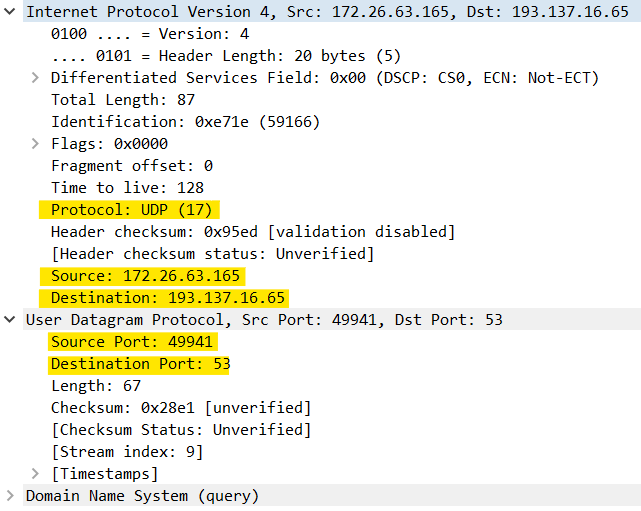
\includegraphics[scale=0.65]{PDU.png}
    \centering
    \caption{Exemplificação de PDU.}
    \label{fig:PDU}
    \end{figure}
\end{enumerate}


\begin{enumerate}[\textbf{b)}]
  \item \textbf{Utilizando o sniffer em modo de captura, proceda à invocação de várias aplicações conhecidas, nomeadamente:}
  \vspace{5mm}
  \begin{itemize}
      \item Acesso via browser ao URL: http://marco.uminho.pt
      \item Acesso ftp (anonymous): ftp.di.uminho.pt
      \item Acesso em tftp para router-ext (193.136.9.33)
      \item Acesso via telnet para router-ext (193.136.9.33) ou para\\*
      router-lab (192.168.90.254)
      \item Acesso ssh para qualquer host da sala de aula
      \item Resolução de nomes usando nslookup www.uminho.pt
      \item traceroute cisco.uminho.pt
  \end{itemize}
  \par \textbf{e construa uma tabela onde, para cada aplicação, conste o protocolo de transporte e a porta de atendimento do
  servidor (quando aplicável).}
  
  % Start new paragraph using alignment Justification 
  \vspace{5mm}
   
  \begin{table}[h!]
    \centering
    \begin{tabular}{p{4.4cm}  p{3cm}  p{3cm}} 
     \hline
     \textbf{Protocolo de Transporte} & \textbf{Porta de Origem} & \textbf{Porta de Destino}\\ [1ex] 
     \hline\hline
     HTTP & 6 & 87837 \\ [1ex]
     FTP & 7 & 78 \\ [1ex]
     TFTP &  & 69 \\ [1ex]
     TELNET & 545 & 23 \\ [1ex]
     SSH & 88 & 22 \\ [1ex]
     DNS & 88 & 53 \\ [1ex]
     ICMP & 88 & 53 \\ [1ex] 
     \hline
    \end{tabular}
    \caption{Tabela de aplicações}
    \label{table:1}
    \end{table}


\end{enumerate}


\section{Parte 2 - Filtragem de tráfego}

\begin{enumerate}[\textbf{a)}]
  \item \textbf{Explore e descreva:}
  \begin{enumerate}[i]
    \item A utilidade dos filtros de captura e visualização;    
    \item A sintaxe e semântica dos filtros.
  \end{enumerate}
  \par\textbf{Dê alguns exemplos simples de utilização dos mesmos.}
  \begin{flushleft}
    INICIO RESPOSTA
  \end{flushleft}
\end{enumerate}


\begin{enumerate}[\textbf{b)}]
  \item  \textbf{Baseando-se nas tramas capturadas acima (1.b), e em outros exemplos que achar conveniente, explore a
  utilidade e utilização dos filtros de captura e visualização, nomeadamente na captura/visualização de:}
  \begin{itemize}
    \item protocolos aplicacionais;
    \item protocolos de transporte;
    \item endereços IP;
    \item pacotes com valores específicos nos campos principais dos cabeçalhos de transporte e rede (ver opção
    "+Expression");
    \item pacotes com flags de iniciação e termino de conexões TCP;
  \end{itemize}
  \par \textbf{Exemplifique a exploração que realizou, indicando a sintaxe utilizada nos filtros e, muito sucintamente os
  resultados obtidos.}
  \begin{flushleft}
    INICIO RESPOSTA
  \end{flushleft}
\end{enumerate}


\begin{enumerate}[\textbf{c)}]
  \item \textbf{Para uma das aplicações que usam o protocolo TCP (e.g. Telnet router-ext), explore a opção "Analyse - Follow TCP Stream". Indique os filtros automaticamente aplicados por essa opção. Discuta eventuais fragilidades
  de segurança e confidencialidade dos dados.}
  
  \vspace{5mm}
  \begin{flushleft}
    \par Com a opção de filtragem via menu Analyse > Follow > TCP Stream, é possível selecionar um pacote entra vários capturados e reunir todos os pacotes que pertencem ao mesmo stream de dados. Neste caso foi feito inicialmente uma filtragem pelo protocolo Telnet, conforme visto na figura~\ref{fig:stream1} abaixo:
    \begin{figure}[h]
      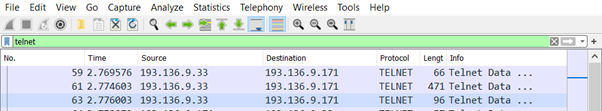
\includegraphics[scale=0.65]{stream1.png}
      \centering
      \caption{Exemplo lista de stream.}
      \label{fig:stream1}
    \end{figure}
  \end{flushleft}

  \begin{flushleft}
    \par Em seguida foi utilizado o menu Analyse > Follow > TCP Stream, mencionado anteriormente e com isso foi possível agrupar todos os pacotes pertencentes ao stream de pacotes pertencentes ao stream do pacote selecionado, inclusive aqueles que não são exclusivamente de protocolo Telnet, conforme visto a seguir na figura~\ref{fig:stream2}.
    \begin{figure}[h]
      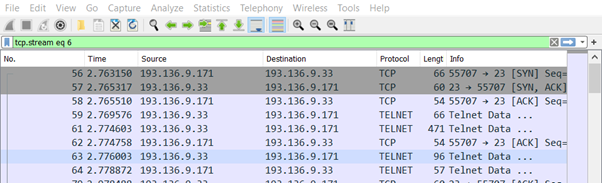
\includegraphics[scale=0.65]{stream2.png}
      \centering
      \caption{Exemplo lista de stream.}
      \label{fig:stream2}
    \end{figure}
  \end{flushleft}

  \begin{flushleft}
    \par Como pode também ser visto na figura~\ref{fig:stream2} o filtro que é gerado pelo menu executado basicamente é filtrar na captura pelo stream TCP de número 6 que sintaticamente possui a expressão (tcp.stream eq 6), o trecho tcp.stream indica intuitivamente que quer se filtrar por streams TCP e a parte (eq 6) indica que o stream especifico que se deseja é o de número igual (eq) a 6.
    \par E o mais interessante do resultado da ação executado pelo menu selecionado é a reconstrução e apresentação das trocas de mensagens trocadas entre origem e destino, de tal forma que seja possível capturar e entender uma troca de mensagens por completo, se forem enviados em texto claro, que é o caso do protocolo Telnet. Tal resultado é visualizado na figura~\ref{fig:followstream}
    \begin{figure}[h]
      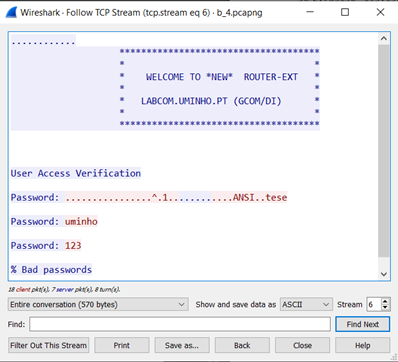
\includegraphics[scale=0.65]{followstream.png}
      \centering
      \caption{Montando o stream.}
      \label{fig:followstream}
    \end{figure}
  \end{flushleft}

  \begin{flushleft}
    \par Os trechos apresentados marcados em azul foram recebidos pelo destinatário e em vermelho pela a origem, que está a tentar aceder ao equipamento via protocolo Telnet. Assim vemos de forma clara o password que foi digitado pelo utilizador. Desta forma mostra a fragilidade do protocolo Telnet, bem como outros protocolos que transmitem suas mensagens via texto claro, caso sejam transmitidos conteúdos sensíveis como senhas, informações bancárias e outros, tais dados estarão expostos e a comprometer a confidencialidade das informações caso haja um utilizador malicioso a sniffar os pacotes que são transmitidos pela rede.
  \end{flushleft}
\end{enumerate}


\begin{enumerate}[\textbf{d)}]
  \item \textbf{Analise e identifique dados estatísticos da sua captura de pacotes.}

  \begin{flushleft}
    Dentre as capturas realizadas selecionou-se a referente ainda ao Telnet. Na tela principal já é possivel verificar a quantidade de pacotes capturados no total e quantos estão sendo exibidos, quando há um filtro aplicado.
    \par CRIAR TABELA AQUI:
    \par Quantidade de pacotes capturados: 352
    \par Total de pacotes exibidos: 50(14.2\%)
    \par Outra opção para se obter mais estatísticas é utilizar o menu Statistics, nele há uma lista de opções. Uma delas que é interessante é o Conversation, nesta são compiladas todas as conversas entre origm X e destindo Y para os protocolos Ethernet, Ipv4, Ipv6, TCP e UDP, sendo essas opções distribuídas em abas, conforme visto abaixo na figura~\ref{fig:conversation01}.
    \begin{figure}[h]
      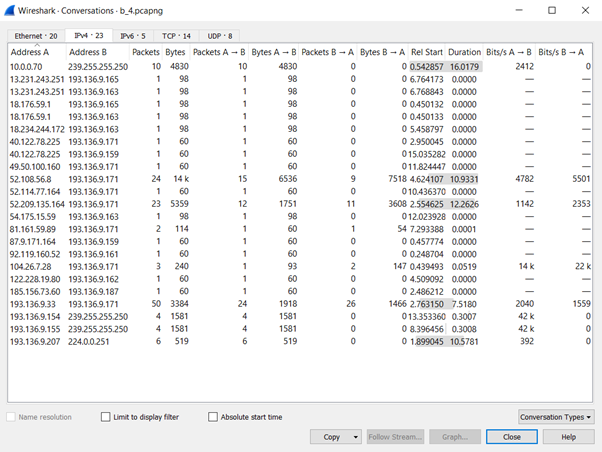
\includegraphics[scale=0.65]{conversation01.png}
      \centering
      \caption{Tabela conversation.}
      \label{fig:conversation01}
    \end{figure}
  \end{flushleft}
\end{enumerate}
\begin{flushleft}
  \par Outra estatistica interessante é listagem hierárquica dos protocolos, nela pode-se ver a representatividade de cada protocolo e subprotocolo no total da captura. Essa estatística pode ser visualizada na figura~\ref{fig:statistic}.
  \begin{figure}[h]
    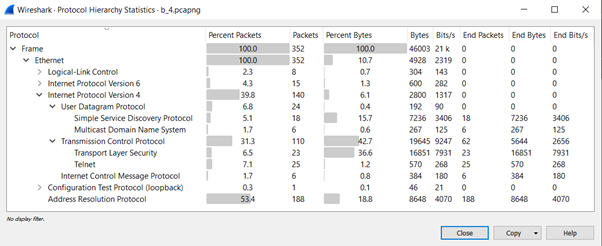
\includegraphics[scale=0.65]{statistic.png}
    \centering
    \caption{Tabela de estatística hierárquica.}
    \label{fig:statistic}
  \end{figure}
\end{flushleft}

\begin{flushleft}
  \par E outra forma de visualizar estatísticas é na opção File Properties do menu Statistics, que pode ser visualizado na figura~\ref{fig:details}
  \begin{figure}[h]
    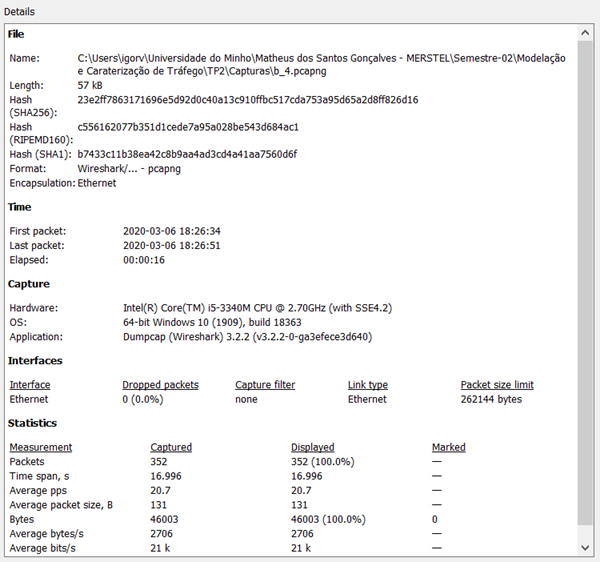
\includegraphics[scale=0.65]{details.png}
    \centering
    \caption{File Properties.}
    \label{fig:details}
  \end{figure}
  \par Quantidade de pacotes capturados: 352
  \par Total de pacotes exibidos: 50(14.2\%)
  
\end{flushleft}

\section{Conclusão}
  \begin{flushleft}
    INICIO CONCLUSAO

  \end{flushleft}

\newpage


% END OFFICIAL REPORT. BELOW THIS MARK IS TRASH AND TESTS.



%
\section{Resultados}
%
Os resultados dos experimentos se encontram na tabela 1. 

\begin{table}
\centering
\begin{tabular}{|c|S|c|c|c|c|c|c|c|c|}
\hline
\multicolumn{3}{|c|}{Parâmetros} & \multicolumn{5}{|c|}{Geração até chegar à solução} & \multicolumn{2}{|c|}{Desempenho} \\ 
\hline
Grade & Mutação & População & \multicolumn{2}{|c|}{95\% de confiança} & 1º Quartil & Mediana & 3º Quartil & Indivíduos & IC \\ 
\hline
3x3 & 0.1 & 10 & 2 & 1000 & 16 & 167 & 435 & 1670 & 96,17\%\\ 
\hline
3x3 & 0.01 & 10 & 1 & 1000 & 12 & 132 & 383 & 1320 & 92,42\%\\ 
\hline
3x3 & 0.001 & 10 & 2 & 1000 & 40 & 197 & 430 & 1970 & 97,87\%\\ 
\hline
3x3 & 0 & 10 & 2 & 1000 & 32 & 135 & 404 & 1350 & 92,85\%\\ 
\hline
3x3 & 0.1 & 100 & 1 & 6 & 2 & 3 & 4 & 300 & 44,37\%\\ 
\hline
3x3 & 0.01 & 100 & 1 & 7 & 2 & 3 & 4 & 300 & 44,37\%\\ 
\hline
3x3 & 0.001 & 100 & 1 & 7 & 2 & 3 & 4 & 300 & 44,37\%\\ 
\hline
3x3 & 0 & 100 & 1 & 8 & 2 & 3 & 4 & 300 & 44,37\%\\ 
\hline
3x3 & 0.1 & 1000 & 1 & 2 & 1 & 1 & 1 & 1000 & 85,84\%\\ 
\hline
3x3 & 0.01 & 1000 & 1 & 2 & 1 & 1 & 1 & 1000 & 85,84\%\\ 
\hline
3x3 & 0.001 & 1000 & 1 & 2 & 1 & 1 & 1 & 1000 & 85,84\%\\ 
\hline
3x3 & 0 & 1000 & 1 & 3 & 1 & 1 & 1 & 1000 & 85,84\%\\ 
\hline
4x4 & 0.1 & 10 & 406 & 1000 & 1000 & 1000 & 1000 & 10000 & \\ 
\hline
4x4 & 0.01 & 10 & 535 & 1000 & 1000 & 1000 & 1000 & 10000 & \\ 
\hline
4x4 & 0.001 & 10 & 241 & 1000 & 1000 & 1000 & 1000 & 10000 & \\ 
\hline
4x4 & 0 & 10 & 185 & 1000 & 1000 & 1000 & 1000 & 10000 & \\ 
\hline
4x4 & 0.1 & 100 & 5 & 27 & 11 & 14 & 17 & 1400 & 2,11\%\\ 
\hline

\hline
\hline\end{tabular}
\label{tab:resultados}
\caption{\small{Resultados brutos}} 
\end{table}

\newpage
\section{Anexo I}
\label{sec:anexo_I}

\begin{table}
\centering
\begin{longtable}{p{.20\textwidth} p{.20\textwidth} p{.20\textwidth} p{.40\textwidth}}
\label{tbl:2}

%\begin{tabular}{p{2cm}|p{2cm}|p{2cm}|p{8cm}}

\\\textbf{Test} & \textbf{Metric} & \textbf{Plataform} & \textbf{Description}\\
\hline\hline
Download (TCP) & Download speed & Whiteboxes, Routers, Android, iOS & The download speed in Mbps when downloading (using TCP) random bytes from a test server \\ 
\hline 
  & TCP Retransmissions & Whiteboxes, Routers & The number of retransmitted TCP segments/packets \\ 
\hline
  & Burst download speed & Whiteboxes, Routers & The download speed during the first 5 seconds of a test \\ 
\hline 
  & Sustained download speed & Whiteboxes, Routers & The download speed of the test during the last 5 seconds \\ 
\hline 
  & Percentage of Best & Whiteboxes, Routers & Download speed result as a percentage of the user's best ever result \\ 
\hline 
  & Percentage of Advertised & Whiteboxes, Routers & Download speed result as a percentage of their package's advertised downstream speed \\ 
\hline 
Download (HTML5) & Download speed & Web & The download speed in Mbps when downloading (using TCP) random bytes from a test server using HTML5 APIs(WebSockets and Fetch) \\ 
\hline 
Download (Lightweight UDP) & Download speed & Whiteboxes, Routers & The download speed in Mbps when downloading (using UDP) from a test server, using less data than the TCP test \\ 
\hline 
Download (Hardware acceleratedUDP) & Download speed & Broadcom-based Routers & The download speed in Mbps when downloading (using UDP) random bytes from a test server \\
\hline 
\caption{Tabela com alguns exemplos}
\end{longtable}
\end{table}
%
%\section{Conclusões}
%
\par O experimento é pequeno para mostrar dados conclusivos, mas mostra indícios do comportamento dos parâmetros de maneira bastante consistente. Obviamente, alterações no algoritmo ou alterações na forma como o problema é representado devem alterar esse comportamento.

Futuros trabalhos podem ser feitos usando-se uma metodologia parecida, mas com modificações no algoritmo e no problema para validar os dados aqui obtidos.

%
% ---- Bibliography ----
%
\begin{thebibliography}{5}
%

\bibitem {castro}
de Castro, L.N.: Fundamentals of Natural Computing: Basic Concepts, Algorithms, and Applications. CRC Press (2006).

\bibitem{racket}
Felleisen, M., Findler, R.B., Flatt, M.: The Racket Manifesto. LIPIcs-Leibniz. (2015).

\bibitem{deb:agra}
Deb, K., Agrawal, S.: Understanding interactions among genetic algorithm parameters. Foundations of Genetic Algorithms. (1999).

\end{thebibliography}

\end{document}
